An early and quite sophisticated version of what we now call a parachute is described in Leonardo's Codex Atlanticus (ca. 1485). Leonardo's parachute consisted of a sealed linen cloth held open by a pyramid-shaped wooden structure.

\bf{Linked rings}

Skydiver Adrian Nicholas tested Leonardo's design more than 500 years later. For this, a modern lightweight structure tied Leonardo's parachute to the human body. We want to use linked rings, which also provide hooks for the sealed linen cloth. Each ring is made of flexible and strong material. Rings can be easily linked together as every ring can be opened and re-closed. A special configuration of linked rings is the chain. A chain is a sequence of rings in which each ring is only connected to its (at most two) neighbours, as illustrated below. This sequence must have a start and an end (rings that are connected to at most one other ring each). Specifically, a single ring is also a chain.

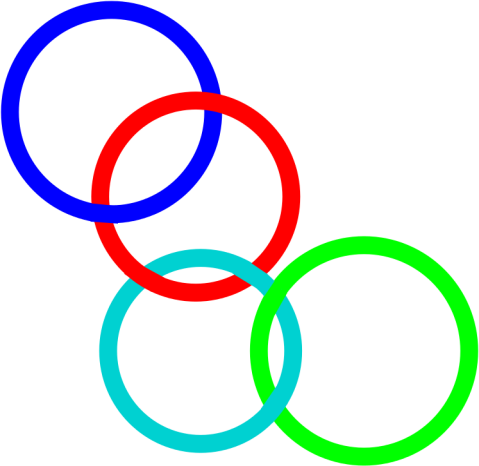
\includegraphics{image_000.png}

Other configurations are clearly possible, since a ring can be linked to three or more other rings. We say that a ring is critical if after opening and removing it, all remaining rings form a set of chains (or there are no other rings left). In other words, there can be nothing but chains left.

\bf{Example}

Consider the seven rings in the next figure, numbered from $0$ to $6$. There are two critical rings. One critical ring is $2$: after its removal, the remaining rings form chains $[1]$, $[0, 5, 3, 4]$ and $[6]$. The other critical ring is $3$: after its removal, the remaining rings form chains $[1, 2, 0, 5]$, $[4]$ and $[6]$. If we remove any other ring, we do not obtain a set of disjoint chains. For example, after removing ring $5$: although we have that $[6]$ is a chain, the linked rings $0, 1, 2, 3$ and $4$ do not form a chain.

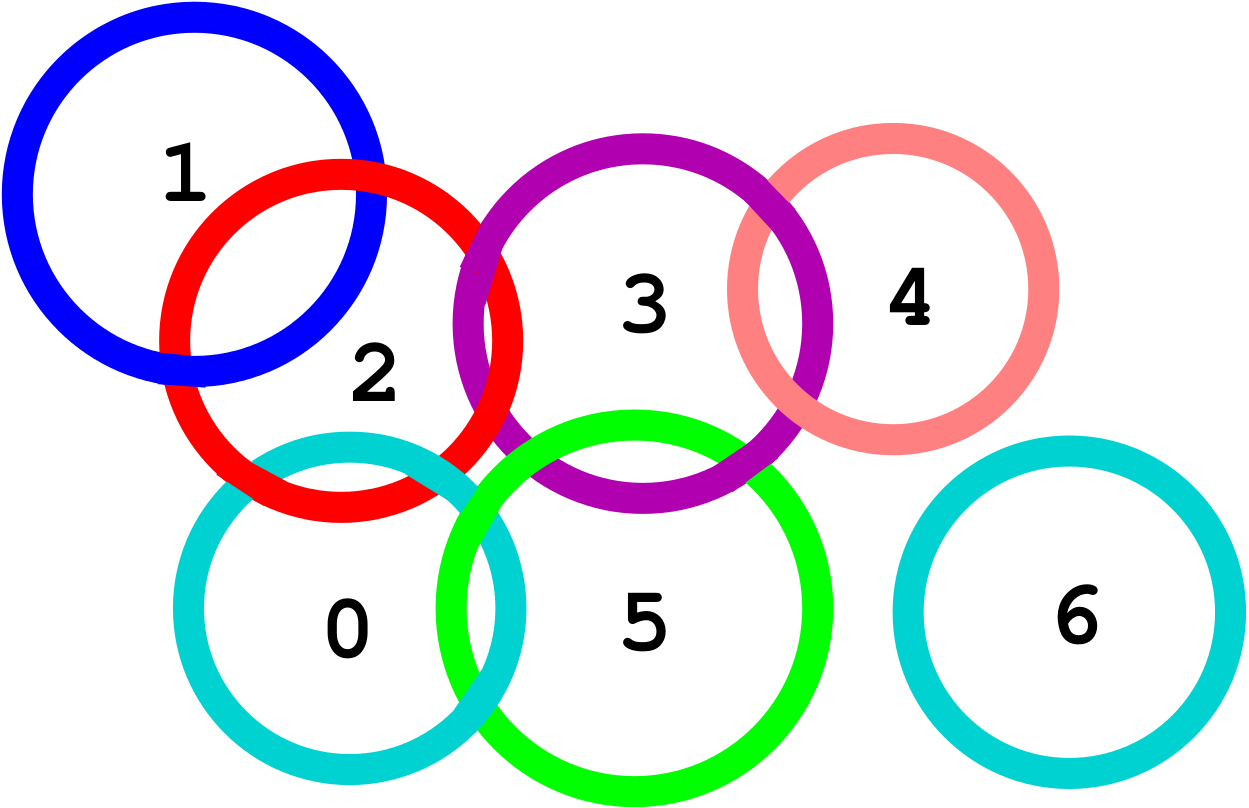
\includegraphics{image_001.png}

\bf{Statement}

Your task is to count the number of critical rings in a given configuration that will be communicated to your program.

At the beginning, there are a certain number of disjoint rings. After that, rings are linked together. At any given time, you can be asked to return the number of critical rings in the current configuration. Specifically, you have to implement three routines.

\begin{itemize}
\item \t{Init(N)} --- it is called exactly once at the beginning to communicate that there are $N$ disjoint rings numbered from $0$ to $N - 1$ (inclusive) in the initial configuration.
\item \t{Link(A, B)} --- the two rings numbered $A$ and $B$ get linked together. It is guaranteed that $A$ and $B$ are different and not already linked directly; apart from this, there are no additional conditions on $A$ and $B$, in particular no conditions arising from physical constraints. Clearly, \t{Link(A, B)} and \t{Link(B, A)} are equivalent.
\item \t{CountCritical()} --- return the number of critical rings for the current configuration of linked rings.
\end{itemize}

You have to submit exactly one file, called \t{rings.c}, \t{rings.cpp} or \t{rings.pas}. This file implements the subprograms described above using the following signatures.

C/C++ programs:

\begin{itemize}
\item \t{void Init(int N);}
\item \t{void Link(int A, int B);}
\item \t{int CountCritical();}
\end{itemize}

Pascal programs:

\begin{itemize}
\item \t{procedure Init(N : LongInt);}
\item \t{procedure Link(A, B : LongInt);}
\item \t{function CountCritical() : LongInt;}
\end{itemize}
These subprograms must behave as described above. Of course you are free to implement other subprograms for their internal use. Your submissions must not interact in any way with standard input/output, nor with any other file.


\bf{Sample grader}

The sample grader reads the input in the following format:
\begin{itemize}
\item line 1: $N$, $L$;
\item lines 2, \dots, L + 1:
\begin{itemize}
\item $-1$ to invoke \t{CountCritical};
\item $A$, $B$ parameters to invoke \t{Link} with $A$ and $B$ as parameters.
\end{itemize} \end{itemize}
The sample grader will print all results from \t{CountCritical}.